% !TEX root = ./Decompositon_Fusion_Rule.tex
\documentclass{beamer}

\usepackage{amsmath}
\usepackage{amssymb}
\usepackage{bm}
\usepackage{adjustbox}  % Để scale bảng và công thức không tràn slide
\usepackage{graphicx}   % Để chèn hình ảnh
\usepackage[utf8]{inputenc}
\usepackage[T5]{fontenc}
\usepackage[vietnamese]{babel}

\usetheme{hust}

\title{Hợp Nhất Ảnh Y Tế Đa Modal}
\subtitle{Phương pháp Phân tích Ảnh và Quy tắc Hợp nhất}
\author{Đỗ Trung Kiên}
\institute{Đại học Bách khoa Hà Nội}
\date{\today}

\begin{document}

\frame{\titlepage}

\begin{frame}{Nội dung trình bày}
    \tableofcontents
\end{frame}

% ============================================================
\section{Tổng quan về Phân tích và Tái tạo ảnh}
% ============================================================

\begin{frame}{Tổng quan về Phân tích và Tái tạo ảnh}
    Trong hợp nhất ảnh y tế đa modal, quá trình \textbf{phân tích} (decomposition) và \textbf{tái tạo} (reconstruction) quyết định chất lượng ảnh hợp nhất.

    \vspace{0.3cm}
    \textbf{Mục tiêu chính:}
    \begin{enumerate}
        \item \textbf{Phân tích} ảnh gốc thành các thành phần con (miền không gian, tần số, thang độ...).
        \item \textbf{Kết hợp} (fuse) các thành phần theo quy tắc phù hợp.
        \item \textbf{Tái tạo} thành ảnh hợp nhất giữ được thông tin từ tất cả modal (MRI+CT, PET+MRI...).
    \end{enumerate}

    \vspace{0.3cm}
    \begin{block}{Quy trình tổng quát}
        Image Decomposition $\to$ Image Fusion Rules $\to$ Image Reconstruction
        \\[0.2cm]
        \footnotesize{Kèm đánh giá chất lượng: MI, PSNR, SSIM...}
    \end{block}
\end{frame}

\begin{frame}{6 Phương pháp phân tích chính}
    \begin{table}
        \centering
        \renewcommand{\arraystretch}{1.2}
        \resizebox{\textwidth}{!}{%
        \begin{tabular}{|l|c|c|c|c|c|c|}
            \hline
            \textbf{Phương pháp} & \textbf{Spatial} & \textbf{Freq.} & \textbf{Multi-} & \textbf{Scale} & \textbf{Dict.} & \textbf{Dir.} \\
            & \textbf{domain} & \textbf{domain} & \textbf{scale} & \textbf{invar.} & & \textbf{filter} \\ \hline
            Color space   & \checkmark & $\times$ & $\times$ & $\times$ & $\times$ & $\times$ \\ \hline
            Pyramid       & $\times$ & \checkmark & \checkmark & $\times$ & $\times$ & $\times$ \\ \hline
            Wavelet       & $\times$ & \checkmark & \checkmark & \checkmark & $\times$ & \checkmark \\ \hline
            Geometric     & $\times$ & \checkmark & \checkmark & \checkmark & $\times$ & \checkmark \\ \hline
            Sparse rep.   & \checkmark & \checkmark & $\times$ & $\times$ & \checkmark & $\times$ \\ \hline
            Salient feat. & \checkmark & $\times$ & \checkmark & \checkmark & $\times$ & $\times$ \\ \hline
        \end{tabular}}
        \caption{So sánh 5 phương pháp phân tích ảnh (Table 1)}
    \end{table}
\end{frame}

% ============================================================
\section{Các phương pháp phân tích ảnh}
% ============================================================

\subsection{2.1. Nhóm Không gian màu (Color Space)}

\begin{frame}{2.1. Phương pháp Color Space}
    \begin{columns}[T]
        \begin{column}{0.38\textwidth}
            \small
            \textbf{Đặc điểm:} Phổ biến nhất là \textbf{IHS} (Intensity-Hue-Saturation) -- cho ra ảnh màu sắc đẹp, tự nhiên.

            \vspace{0.15cm}
            \textbf{Phù hợp y tế?} Ảnh y tế thường là \textit{pseudo-color}.

            \vspace{0.15cm}
            \textbf{Quy trình IHS Fusion:}
            \begin{enumerate}
                \item RGB $\to$ IHS.
                \item Giữ $H$, $S$; thay $I$ bằng ảnh kia.
                \item IHS $\to$ RGB ra $I_F$.
            \end{enumerate}
            \normalsize
        \end{column}
        \begin{column}{0.60\textwidth}
            \centering
            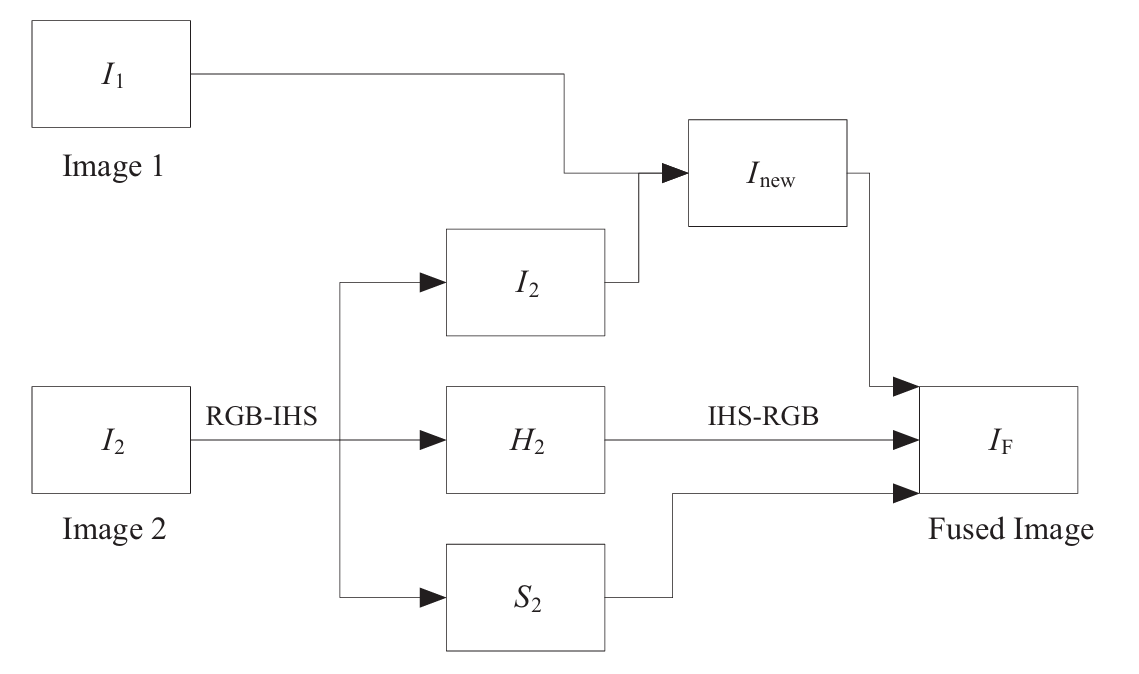
\includegraphics[width=\linewidth]{../Slide/DATN/Week_3/Image_Decomposition/IHS-basedfusion.png}
            \\[2pt]
            {\footnotesize\textit{Pipeline IHS-based Fusion}}
        \end{column}
    \end{columns}
\end{frame}

\begin{frame}{Công thức RGB $\to$ IHS}
    \begin{block}{Intensity và Saturation}
    \begin{equation}
        I = \frac{R + G + B}{3}, \qquad S = 1 - \frac{3\min(R,G,B)}{R+G+B}
    \end{equation}
    \end{block}

    \begin{block}{Thành phần Hue $(H)$}
    \begin{align}
        H &= \begin{cases}
            \theta & \text{nếu } B \leq G \\
            360^\circ - \theta & \text{nếu } B > G
        \end{cases}\nonumber\\
        \theta &= \cos^{-1}\!\left(\frac{(R-G)+(R-B)}{2\sqrt{(R-G)^2+(R-B)(G-B)}}\right)
    \end{align}
    \end{block}
\end{frame}

\begin{frame}{Công thức IHS $\to$ RGB (chuyển ngược)}
    \begin{block}{Chuyển ngược IHS $\to$ RGB}
    \begin{align}
        R &= I + S\cos(H) \nonumber\\
        G &= I + S\cos(120^\circ - H) \\
        B &= I + S\cos(240^\circ - H) \nonumber
    \end{align}
    \end{block}

    \vspace{0.3cm}
    \begin{block}{Ghi chú}
        Hợp nhất IHS: giữ $H$, $S$ từ ảnh 1; thay $I$ bằng ảnh 2 (hoặc weighted average), sau đó chuyển ngược về RGB.
    \end{block}
\end{frame}

\begin{frame}{Đánh giá Color Space}
    \begin{columns}
        \begin{column}{0.5\textwidth}
            \textbf{Ưu điểm:}
            \begin{itemize}
                \item Đơn giản, dễ hiểu.
                \item Giữ được màu sắc đẹp và tự nhiên.
                \item Phù hợp ảnh y tế pseudo-color.
            \end{itemize}
        \end{column}
        \begin{column}{0.5\textwidth}
            \textbf{Nhược điểm:}
            \begin{itemize}
                \item \textbf{Không có multi-scale} -- chỉ xử lý ở một độ phân giải.
                \item Dễ mất thông tin \textbf{tần số cao} (chi tiết nhỏ, cạnh sắc nét).
            \end{itemize}
        \end{column}
    \end{columns}
\end{frame}

\subsection{2.2. Nhóm Phân rã Đa tỉ lệ (Multi-scale - MSD/MGD)}

\begin{frame}{Tầm quan trọng của Phân rã Đa tỉ lệ (MSD)}
    \small
    \textbf{Tại sao cần Đa tỉ lệ?} 
    Ảnh y tế chứa thông tin ở nhiều mức độ chi tiết (cấu trúc lớn, mô mềm, mạch máu nhỏ...). 
    Phân rã đa tỉ lệ giúp trích xuất các thành phần này một cách hiệu quả.

    \vspace{0.2cm}
    \textbf{Lợi ích chính:}
    \begin{itemize}
        \item Khả năng trích xuất cấu trúc không gian qua các thang đo khác nhau.
        \item Giảm thiểu sự dư thừa thông tin giữa các modal.
        \item Phù hợp với cơ chế thị giác của con người (HVS).
    \end{itemize}

    \vspace{0.3cm}
    \begin{block}{Sự tiến hóa của MSD}
        Pyramid (Tuyến tính) $\to$ Wavelet (Tần số) $\to$ MGD (Geometric: Hướng \& Cạnh)
    \end{block}
\end{frame}

\begin{frame}{2.2.1. Phương pháp Pyramid}
    \small
    \textbf{Đặc điểm:} Quá trình phân tách bao gồm việc \textbf{lọc (filtering)} và \textbf{giảm mẫu (down-sampling)} liên tiếp, tạo ra các bản sao thông dải và thông thấp.
    \begin{equation}
        R_i = F_i * P_i; \quad P_{i+1} = P_i - R_i; \quad I_{rec} = P_{L+1} + \sum_{i=1}^L R_i
    \end{equation}
    ($R_i$: residual, $F_i$: filter, $P_i$: pyramid representation)

    \vspace{0.2cm}
    \textbf{Các loại phổ biến:} Laplacian [11], Gradient [16], Morphological [41], Steerable [42], Ratio [38].

    \vspace{0.2cm}
    \begin{alertblock}{Hạn chế quan trọng}
        Cơ chế không phân định hướng (\textit{non-orientation}), gây ra \textbf{blocking effects} (hiệu ứng khối) và tạo ra các cạnh không mong muốn (\textit{undesired edges}), không giữ được thông tin salient dưới tác động của nhiễu.
    \end{alertblock}
\end{frame}



\begin{frame}{2.2.2. Phương pháp Wavelet (Biến đổi Sóng con)}
    \begin{columns}[T]
        \begin{column}{0.45\textwidth}
            \small
            \textbf{Cấu trúc:} Kết hợp hai nhóm hàm: \textit{wavelet functions} (mẹ) và \textit{scaling functions}.
            \begin{equation}
                \psi_{a,b}(x) = a^{-1/2} \psi\left(\frac{x-b}{a}\right)
            \end{equation}
            \textbf{Ưu điểm vượt trội:}
            \begin{itemize}
                \item Bảo toàn thông tin tốt.
                \item Tách biệt tốt tần số cao/thấp.
                \item Linh hoạt với nhiều độ phân giải khác nhau.
            \end{itemize}
            \normalsize
        \end{column}
        \begin{column}{0.53\textwidth}
            \small
            \textbf{Các cải tiến (Advanced WT):}
            \begin{itemize}
                \item \textbf{DWT}: Thiếu tính bất biến dịch chuyển (\textit{shift-invariance}) do down-sampling.
                \item \textbf{RDWT/SWT}: Khắc phục tính bất biến dịch chuyển.
                \item \textbf{DTCWT}: Hỗ trợ 6 hướng, gần như bất biến dịch chuyển.
                \item \textbf{QWT}: Magnitude bất biến dịch chuyển và pha giàu thông tin hình học.
            \end{itemize}
            \normalsize
        \end{column}
    \end{columns}
\end{frame}

\begin{frame}{2.2.3. MGD: Ridgelet \& Curvelet}
    \small
    \textbf{Mục tiêu:} Khắc phục hạn chế của Wavelet trong việc biểu diễn các đặc trưng bất đẳng hướng và các đường chuyển tiếp sắc nét (cạnh).

    \vspace{0.2cm}
    \textbf{Ridgelet Transform (RT):}
    \begin{itemize}
        \item Biểu diễn thưa các đối tượng có \textbf{gián đoạn trên đường thẳng}.
        \item Là phân tích wavelet trong miền \textit{Radon}.
        \item Phù hợp cho việc phát hiện hình dạng và đường thẳng.
    \end{itemize}

    \vspace{0.2cm}
    \textbf{Curvelet Transform (CVT):}
    \begin{itemize}
        \item Tiến hóa từ Ridgelet để xử lý tốt các \textbf{đường cong}.
        \item Tuân theo quy luật tỷ lệ parabol: $width = length^2$.
        \item Gen-2 (Wrapping algorithm) nhanh hơn và giảm dư thừa.
    \end{itemize}
\end{frame}

\begin{frame}{2.2.4. MGD: Contourlet}
    \small
    \textbf{Cấu trúc (CRT):} Kết hợp \textbf{Laplacian Pyramid} (bắt điểm gián đoạn) và \textbf{Directional Filter Bank} (liên kết điểm thành cấu trúc tuyến tính).
    
    \vspace{0.2cm}
    \textbf{Đặc điểm nổi bật:}
    \begin{itemize}
        \item Bắt được các đặc trưng hình học nội tại (contours).
        \item Phân chia 8 hướng cơ bản (và nhiều hơn ở các mức cao).
    \end{itemize}

    \vspace{0.2cm}
    \begin{block}{Non-subsampled Contourlet (NSCT)}
        Biến thể \textbf{bất biến dịch chuyển hoàn toàn} nhờ loại bỏ quá trình down/up-sampling. NSCT cực kỳ hiệu quả trong việc duy trì độ sáng cục bộ và giảm biến dạng trong ảnh CT/MRI.
    \end{block}
\end{frame}

\begin{frame}{2.2.5. State-of-the-Art: Shearlet Transform}
    \small
    \textbf{Ý tưởng:} Tiến hóa từ Curvelet, thay thế directional filter bằng \textbf{shear filter}.
    \begin{equation}
        \psi_{a,s,t}(x) = a^{-3/4} \psi(A_a^{-1} S_s^{-1} (x-t))
    \end{equation}
    ($A_a$: parabolic scaling, $S_s$: shear matrix)

    \vspace{0.2cm}
    \textbf{Tại sao Shearlet tốt nhất?}
    \begin{itemize}
        \item \textbf{Anisotropic shear:} Kiểm soát độ nhạy hướng cực tốt.
        \item \textbf{Tối ưu thưa (Optimally sparse):} Biểu diễn các đường chuyển tiếp sắc nét vượt trội so với Wavelet/Contourlet.
        \item \textbf{Đa hướng:} Số lượng hướng ở mỗi mức là không giới hạn.
    \end{itemize}

    \vspace{0.2cm}
    \begin{exampleblock}{NSST (Non-subsampled Shearlet)}
        Loại bỏ hiện tượng \textbf{Gibbs} do quá trình lấy mẫu, là lựa chọn hàng đầu cho các tác vụ hợp nhất ảnh y tế hiện nay.
    \end{exampleblock}
\end{frame}

\subsection{2.3. Nhóm Hiện đại & Đặc trưng (Modern Methods)}

\begin{frame}{2.3.1. Phương pháp Sparse Representation}
    \small
    \textbf{Ý tưởng:} Ảnh chia sẻ cùng tập \textbf{hệ số thưa} (compressed sensing).
    \quad
    \textbf{Pipeline JSR:}
    (1) Sliding window $\to$ vectorize\;
    (2) Joint sparse: $V = DS_C, DS_U$\;
    (3) Fusion rules\;
    (4) Dict $\to$ Reconstruct $\to$ $I_F$
    \quad\textbf{Ưu:} Chống nhiễu, giữ cấu trúc.\;\textbf{Nhược:} Phụ thuộc từ điển.
    \normalsize

    \vspace{0.15cm}
    \centering
    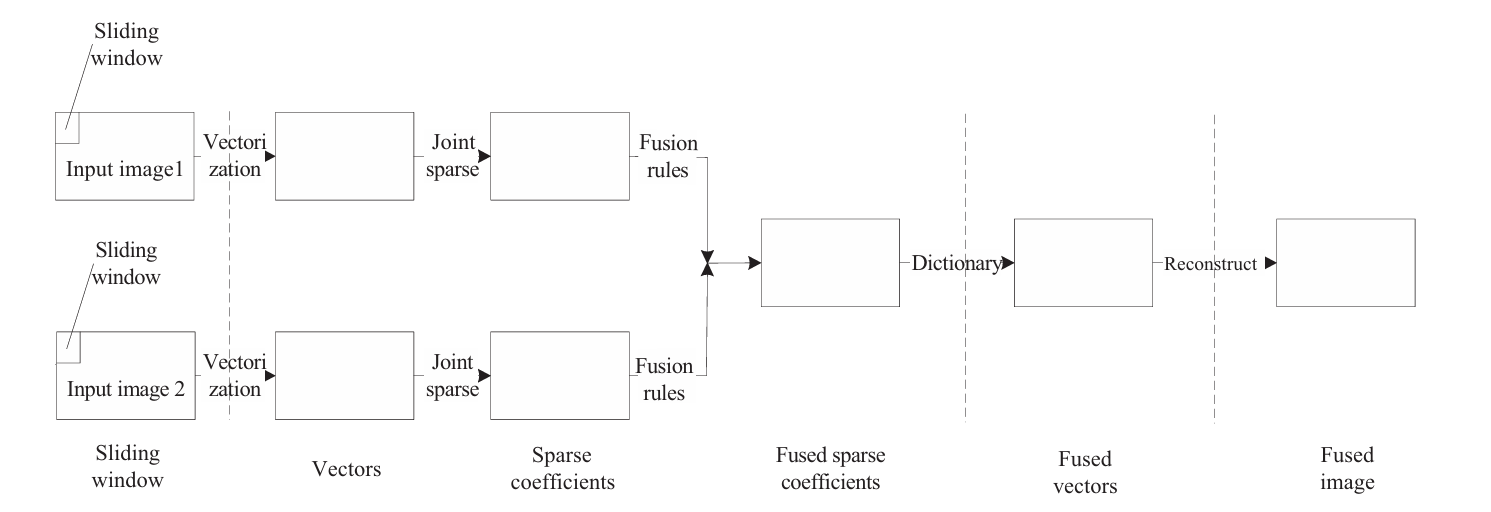
\includegraphics[width=\textwidth,height=0.52\textheight,keepaspectratio]{../Slide/DATN/Week_3/Image_Decomposition/jointsparserepresentation.png}
    \\[2pt]
    {\footnotesize\textit{Pipeline Joint Sparse Representation}}
\end{frame}

\begin{frame}{2.3.2. Phương pháp Salient Feature}
    \small
    \textbf{Đặc điểm:} Spatial domain, dùng \textbf{edge-preserving filters} tách base/detail layer đa thang.
    \quad
    \textbf{Pipeline:}
    (1)\;$B_i = I*F_i,\; D_i = I - B_i$\;
    (2) Fuse: $B_F = f_B(B_1,B_2),\; D_F = f_D(D_1,D_2)$\;
    (3)\;$I_F = B_F + D_F$
    \quad\textbf{Ưu:} Giữ cạnh, nhanh.\;\textbf{Nhược:} Không có freq. domain.
    \normalsize

    \vspace{0.15cm}
    \centering
    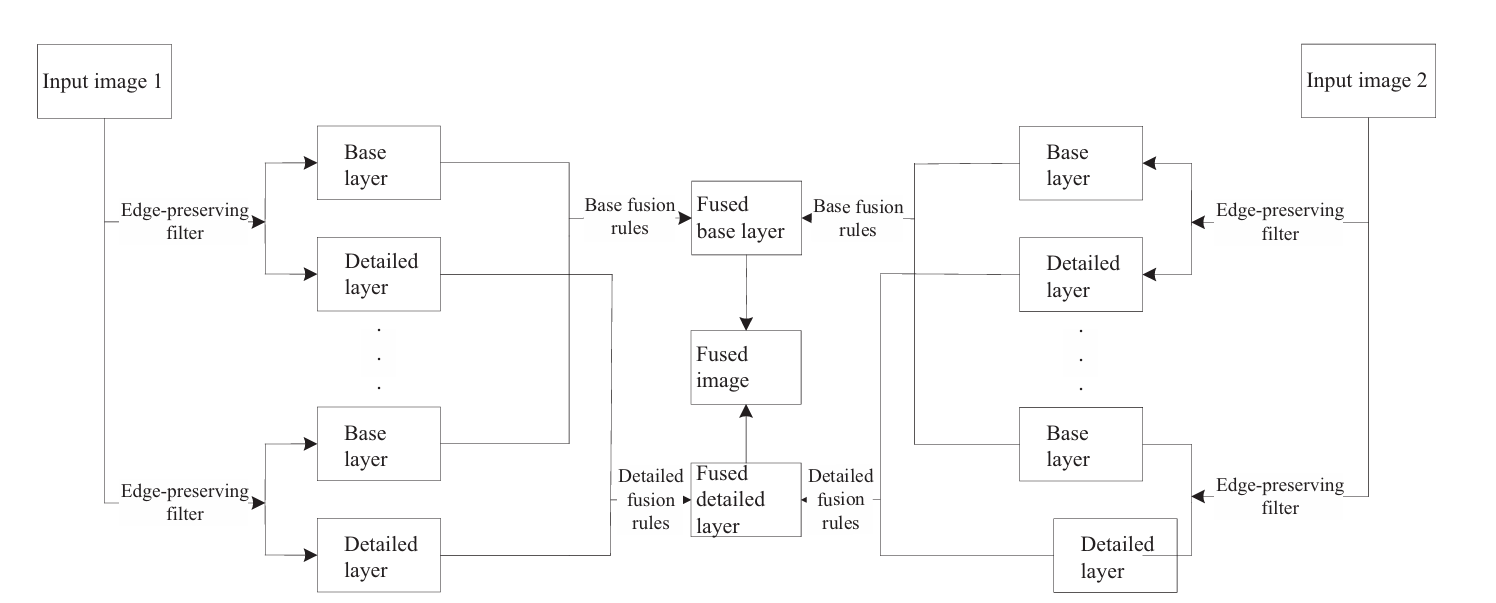
\includegraphics[width=\textwidth,height=0.52\textheight,keepaspectratio]{../Slide/DATN/Week_3/Image_Decomposition/edge-preservingfilter.png}
    \\[2pt]
    {\footnotesize\textit{Pipeline Edge-Preserving Filter Fusion}}
\end{frame}

\begin{frame}{Kết luận phần Decomposition}
    \begin{table}
        \centering
        \small
        \renewcommand{\arraystretch}{1.2}
        \begin{tabular}{|l|p{6.5cm}|}
            \hline
            \textbf{Phương pháp} & \textbf{Đặc điểm nổi bật} \\ \hline
            Color Space  & Đơn giản, đẹp màu, không multi-scale. \\ \hline
            Pyramid      & Đa độ phân giải, hạn chế bởi hiếu hiệu ứng khối. \\ \hline
            Wavelet      & Bảo toàn thông tin, linh hoạt đa độ phân giải. \\ \hline
            Geometric    & \textbf{Tốt nhất} cho đường cong, cạnh và contours. \\ \hline
            Sparse Rep.  & Biểu diễn thưa, chống nhiễu, từ điển học được. \\ \hline
            Salient Feat.& Spatial domain, giữ cạnh, nhanh, sát lâm sàng. \\ \hline
        \end{tabular}
    \end{table}
\end{frame}

% ============================================================
\section{Quy tắc Hợp nhất (Fusion Rules)}
% ============================================================

\begin{frame}{Tổng quan về Image Fusion Rules}
    \textbf{Định nghĩa:} Fusion rules quyết định cách \textbf{kết hợp thông tin} từ nhiều ảnh gốc thành ảnh hợp nhất, nhấn mạnh đặc trưng quan trọng và kìm hãm đặc trưng không quan trọng.

    \vspace{0.3cm}
    \textbf{4 thành phần của một quy tắc hợp nhất điển hình:}
    \begin{enumerate}
        \item \textbf{Activity-level measurement:} Đo mức độ hoạt động/saliency của hệ số.
        \item \textbf{Coefficient grouping:} Nhóm hệ số.
        \item \textbf{Coefficient combination:} Kết hợp hệ số.
        \item \textbf{Consistency verification:} Xác nhận tính nhất quán trong vùng lân cận.
    \end{enumerate}

    \vspace{0.3cm}
    \textbf{3 mức độ triển khai:}
    \begin{itemize}
        \item \textbf{Pixel level:} Dựa trực tiếp vào giá trị pixel.
        \item \textbf{Feature level:} Dựa vào vùng/đặc trưng (saliency, texture...).
        \item \textbf{Decision level:} Dựa trên thống kê, fuzzy logic, machine learning.
    \end{itemize}
\end{frame}

\subsection{Fuzzy Logic (Logic mờ)}

\begin{frame}{3.1. Fuzzy Logic}
    \textbf{Bản chất:} Decision level -- xử lý vấn đề hình ảnh bị mờ (blurry).

    \vspace{0.2cm}
    \textbf{Hai mô hình chính:} Mamdani (cổ điển) và \textbf{Takagi-Sugeno (T-S)} (chính xác hơn, tránh bước defuzzification phức tạp).

    \vspace{0.2cm}
    \textbf{Quy trình:}
    \begin{enumerate}
        \item Trích xuất đặc trưng $C_1, C_2$ từ hai ảnh.
        \item Áp dụng luật IF-THEN:
        \begin{itemize}\small
            \item R1: IF $C_1$ \textit{high} AND $C_2$ \textit{high} THEN $C_w$ \textit{high}
            \item R2: IF $C_1$ \textit{low} AND $C_2$ \textit{high} THEN $C_w$ \textit{medium}
            \item R4: IF $C_1$ \textit{low} AND $C_2$ \textit{low} THEN $C_w$ \textit{low}
        \end{itemize}\normalsize
        \item Tính hàm thuộc Gaussian:
    \end{enumerate}
    \begin{equation}
        \mu_{w_i}(y) = e^{-\frac{(y-\mu_i)^2}{2\sigma_i^2}}, \quad i=1,2,3 \;(\text{high, medium, low})
    \end{equation}
    \begin{enumerate}
        \setcounter{enumi}{3}
        \item Defuzzification bằng \textit{center average} $\to$ trọng số pixel.
    \end{enumerate}
\end{frame}

\subsection{Statistics (Thống kê)}

\begin{frame}{3.2. Statistics -- PCA}
    \textbf{Principal Component Analysis (PCA):} Giảm chiều, tạo trọng số từ thành phần chính.

    \vspace{0.2cm}
    \textbf{Quy trình:}
    \begin{enumerate}
        \item Vector hóa hệ số:
        \begin{equation}
            C_1 = [x_{1,1},\ldots,x_{1,N}]^T, \quad C_2 = [x_{2,1},\ldots,x_{2,N}]^T
        \end{equation}
        \item Ma trận hiệp phương sai:
        \begin{equation}
            \text{Cov}(C_1,C_2) = E\left[(C_1-\mu_1)(C_2-\mu_2)^T\right]
        \end{equation}
        \item Tính trọng số từ eigenvalues $V$ của Cov:
        \begin{equation}
            w_1 = \frac{V_{1,1}}{V_{1,1}+V_{2,1}}, \quad w_2 = \frac{V_{2,1}}{V_{1,1}+V_{2,1}}
        \end{equation}
        \item Hệ số hợp nhất: $C_F = w_1 C_1 + w_2 C_2$
    \end{enumerate}
\end{frame}

\begin{frame}{3.2. Statistics -- Hidden Markov Tree (HMT)}
    \textbf{HMT:} Mô hình hóa hệ số bằng \textit{mixture of two Gaussians} (hai trạng thái ẩn: 0 và 1).

    \vspace{0.2cm}
    \textbf{Cấu trúc:} Quad-tree gồm parent (PC), neighbor (NC), co-located child (CC).

    \vspace{0.2cm}
    \textbf{Xác suất chuyển trạng thái:}
    \begin{equation}
        P = \begin{bmatrix} p_{11} & p_{12} \\ p_{21} & p_{22} \end{bmatrix}
    \end{equation}

    \textbf{Quy tắc hợp nhất:}
    \begin{equation}
        C_F = \begin{cases} C_1 & \text{nếu } C_1 \geq C_2 \\ C_2 & \text{ngược lại} \end{cases}
    \end{equation}

    \vspace{0.1cm}
    \textbf{Ưu điểm:} PCA đơn giản; HMT giữ cấu trúc không gian tốt.\\
    \textbf{Nhược điểm:} PCA có thể mất thông tin phi tuyến.
\end{frame}

\subsection{Human Visual System (HVS)}

\begin{frame}{3.3. Human Visual System (HVS)}
    \textbf{Mục tiêu:} Mô phỏng nhận thức hình ảnh của con người -- tập trung vào cạnh, góc, saliency.

    \vspace{0.2cm}
    \textbf{Visibility:} Đo độ sắc nét, chọn max visibility.
    \begin{equation}
        V(x,y) = \sum_{m,n} \frac{|I(x,y) - \mu|}{\mu^\alpha}, \quad \alpha \approx 0.6\text{--}0.7
    \end{equation}

    \textbf{SUSAN:} Trích xuất đặc trưng dựa trên vùng đồng nhất cường độ.
    \begin{equation}
        n(r_o) = \sum \exp\!\left(-\frac{(r-r_o)^2}{2\eta^2}\right)
                      \exp\!\left(-\frac{(F(r)-F(r_o))^2}{T^2}\right)
    \end{equation}
\end{frame}

\begin{frame}{3.3. HVS -- ANN và Retina-Inspired Model}
    \textbf{Artificial Neural Networks (ANN):}
    \begin{itemize}
        \item \textbf{MNN (Mapping Neural Network):} Multi-level fusion.
        \item \textbf{PCNN (Pulse Coupled Neural Network):} Phổ biến cho Wavelet-based fusion.
        \begin{itemize}
            \item Mô phỏng xung đồng bộ ở vỏ não thị giác mèo.
            \item Mỗi pixel tương ứng một neuron: linking + feeding $\to$ threshold $\to$ pulse.
        \end{itemize}
    \end{itemize}

    \vspace{0.3cm}
    \textbf{Retina-Inspired Model (RIM):} Dùng cho IHS decomposition.
    \begin{itemize}
        \item 5 lớp: cone photoreceptors $\to$ spatial extractor $\to$ horizontal cells $\to$ bipolar $\to$ ganglion.
    \end{itemize}
    \begin{equation}
        C_F = f_1 C_1 + f_2 C_2
    \end{equation}
    \footnotesize{($f_1$: high-scale extractor output, $f_2$: horizontal cells output)}

    \normalsize\vspace{0.1cm}
    \textbf{Ưu điểm:} Giữ đặc trưng mà mắt người nhạy cảm (cạnh, texture).\\
    \textbf{Nhược điểm:} PCNN phức tạp tính toán.
\end{frame}

\subsection{Objective Evaluation Metrics}

\begin{frame}{3.4. Objective Evaluation Metrics}
    Dùng làm \textbf{feedback} để cải thiện và tối ưu hóa quy tắc hợp nhất.

    \vspace{0.2cm}
    \begin{itemize}\small
        \item \textbf{Spatial Frequency (SF):}
        $SF = \sqrt{RF^2 + CF^2}$
        \item \textbf{Ratio of Spatial Frequency Error (rSFe):}
        \[
            rSFe = \frac{|SF_F - SF_1|/SF_1 + |SF_F - SF_2|/SF_2}{2}
        \]
        \item \textbf{Wavelet Entropy (WE):}
        $WE = -\sum_j p_j \ln p_j$, \; $p_j = E_j / E_{\text{tot}}$
        \item \textbf{Directive Contrast (DC):}
        $DC(x,y) = I_H(x,y) / I_L(x,y)$
        \item \textbf{Mutual Information (MI):}
        $MI(I_1,I_F) + MI(I_2,I_F)$
    \end{itemize}\normalsize

    \vspace{0.1cm}
    \textbf{Ưu điểm:} Định lượng, khách quan, làm tiêu chí tối ưu.\\
    \textbf{Nhược điểm:} Không phải lúc nào cũng tương quan với nhận thức con người.
\end{frame}

% ============================================================
\section{Tổng kết}
% ============================================================

\begin{frame}{Tổng kết}
    \textbf{Phần 2 -- Decomposition Methods:}
    \begin{itemize}
        \item \textbf{Color space:} Đơn giản, phù hợp pseudo-color, thiếu multi-scale.
        \item \textbf{Pyramid:} Đa độ phân giải, gặp vấn đề blocking artifacts.
        \item \textbf{Wavelet:} Multi-scale mạnh mẽ, tách tần số tốt.
        \item \textbf{Geometric (Shearlet/NSCT):} \textbf{Chất lượng cao nhất} nhờ tối ưu biểu diễn cạnh và contours.
        \item \textbf{Sparse representation:} Biểu diễn thưa, chống nhiễu tốt.
    \end{itemize}

    \vspace{0.3cm}
    \textbf{Phần 3 -- Fusion Rules:}
    \begin{itemize}
        \item \textbf{Fuzzy logic \& HVS (PCNN, RIM):} Mạnh ở decision/feature level, xử lý tốt sự không chắc chắn.
        \item \textbf{Statistics (PCA, HMT):} Đơn giản, hiệu quả cho saliency ẩn.
        \item \textbf{Objective metrics:} Đóng vai trò feedback để đánh giá và cải tiến quy tắc.
    \end{itemize}

    \vspace{0.2cm}
    \begin{block}{Ghi nhớ}
        Hệ thống Fusion hoàn chỉnh = \textbf{Decomposition} tối ưu + \textbf{Fusion Rule} phù hợp + \textbf{Reconstruction} chất lượng.
    \end{block}
\end{frame}

\begin{frame}
    \centering
    \Huge \textcolor{hustred}{\textbf{CẢM ƠN THẦY VÀ CÁC BẠN}}
    \vspace{0.5cm}

    \Large \textbf{ĐÃ LẮNG NGHE!}

    \vspace{1cm}
    \normalsize
    \textit{Hỏi và đáp (Q\&A)}
\end{frame}

\end{document}
